\section{Spiral Acquisition}
For dynamic imaging like \gls{fMRI}, acquisition speed is of paramount importance. Currently, most \gls{fMRI} studies are performed with Cartesian \gls{EPI} where multiple lines of k-space is acquired after a single \gls{RF} excitation. In a conventional \gls{EPI}, k-space is sampled in a uniform Cartesian grid to have a quick and simple reconstruction. However, the sampling efficiency can be further improved by employing non-Cartesian trajectories such as spiral\cite{ahnHighSpeedSpiralScanEcho1986}. The smooth curvature of the spiral trajectories achieves faster and efficient sampling by minimizing abrupt k-space jumps and using multiple gradient axis simultaneously. Additionally, spiral imaging offers robustness against motion and flow\cite{nishimuraVelocityKSpaceAnalysis1995}. Despite these advantages, adoption of spiral imaging is slow due to the complex non-Cartesian reconstruction, system imperfections and blurring due to spatial $B_0$ homogeneity\cite{gloverSpiralImagingFMRI2012}. In this work, a 3D encoding scheme called stack-of-spirals \cite{irarrazabalFastThreeDimensional1995} is employed for its suitability with the \gls{bSSFP} acquisition(explained in \cref{sec:bSSFP}). The Cartesian phase encoding orthogonal to spiral encoding direction supports asymmetric \gls{FOV} to achieve high resolution in a thin slab and reduces reconstruction complexity.
\begin{figure}[H]
	\centering
	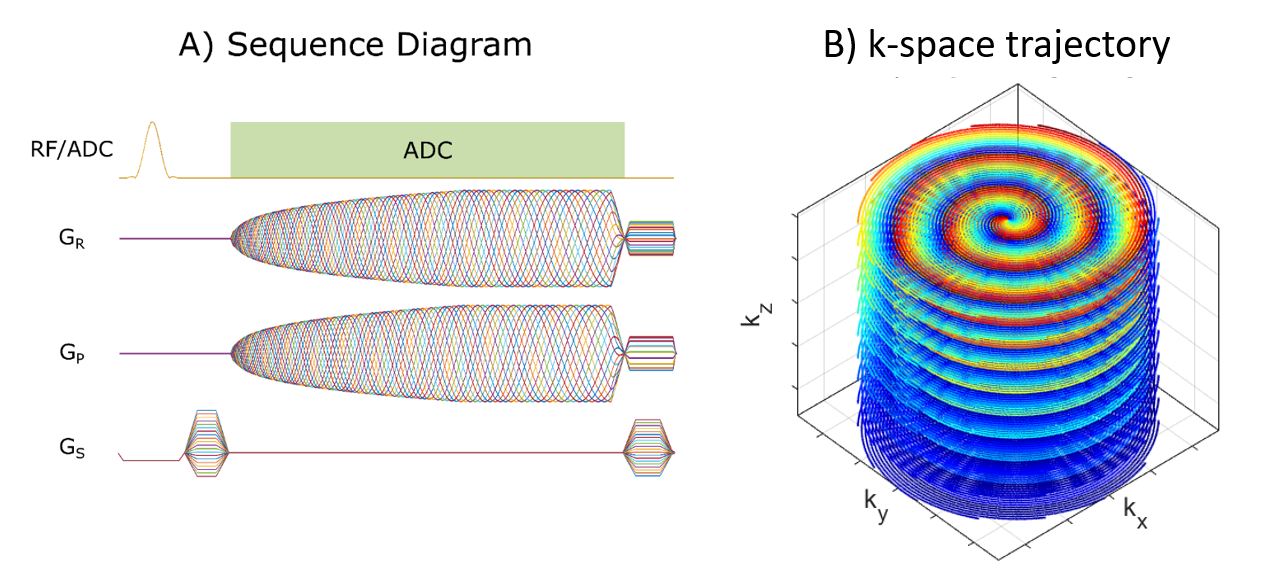
\includegraphics[width=1.0\textwidth]{graphics/sos_seq_traj.png}
	\caption{A 3D \gls{bSSFP} sequence with stack-of-spiral readout in A and the corresponding k-space trajectory in B}
	\label{fig:sos_seq_traj}
\end{figure}
\subsection{Trajectory Design}
The 3D stack-of-spirals trajectory is constructed by rotating and stacking many short spiral interleaves which starts from the k-space center and spirals out as shown in Figure \ref{fig:sos_seq_traj}. A single spiral interleaf is an Archimedian spiral $k(t)$ with uniform density (spiral turns are equidistant) defined as    
\begin{equation}
	k(t)=k_x(t)+jk_y(t)=\lambda\theta e^{j\theta}
\end{equation} 
where $\lambda=N_\text{int}/\text{FOV}$, $N_\text{int}$ is the number of spiral interleaves and $\theta(t)$ is the azimuthal function.  The azimuthal function $\theta(t)$ is calculated to meet both the sampling requirement and the gradient system constraints such as maximum gradient amplitude and maximum slew rate limit. As there is no closed form expression, conventionally spiral gradient waveform is estimated either iteratively or by approximations \cite{gloverSpiralImagingFMRI2012,duynFastSpiralMagnetic1997,gloverSimpleAnalyticSpiral1999}. Here, we used a flexible framework for gradient waveform calculation where Archimedian spiral k-space locations as per sampling requirement is provided to an optimization algorithm. The time-optimal gradient waveform for the input trajectory is estimated for a given gradient constraints\cite{lustigFastMethodDesigning2008}.

\subsection{NUFFT}
The spiral k-space sampling results in a data that doesn't lie on a equidistant Cartesian grid preventing the use of efficient \gls{FFT} algorithm for image reconstruction. To compute Fourier transform of the data sampled on a non-equidistant grid, several efficient \gls{NUFFT} algorithms exists\cite{duttFastFourierTransforms1993} were introduced. The most popular among them is the gridding method where a shift-invariant interpolating kernel is used to regrid the non-equidistant data into an oversampled Cartesian grid followed by efficient \gls{FFT} and removing the blurring introduced by the interpolation kernel through deapodization\cite{jacksonSelectionConvolutionFunction1991}. This use of same shift-invariant kernel throughout the k-space reduces the memory requirement of gridding operation. Ideally, \emph{sinc} kernel gives the exact \gls{DFT} and needs no further no deapodization. However, the large support of \emph{sinc} kernel makes it computationally inefficient. Therefore, trade-off between approximation error and computational complexity of the interpolating kernel has to be reached. The \emph{Kaiser-Bessel} function is a popular choice because of its small approximation error for a relatively small kernel width and oversampling ratio\cite{beattyRapidGriddingReconstruction2005}. The approximation error can be further minimized if an ideal interpolating kernel is estimated from the trajectory. For this reason, the min-max interpolator\cite{fesslerNonuniformFastFourier2003} and its efficient implementation as \emph{Toplitz} matrix\cite{fesslerToeplitzbasedIterativeImage2005} is used in this work.
\subsection{Density compensation}
In addition to \gls{NUFFT}, the sampling density of the trajectory must be compensated to avoid accentuation of some spatial frequencies which are densely sampled. Generally, the densely-sampled low spatial frequencies during the slew-rate limited regime of the spiral trajectory resulting in blurring. When spiral arms have only a few windings, a simple \emph{rho filter} used for the filtered back-projection reconstruction of computed-tomography and radial MR imaging could be used for density compensation. However, density compensation function become non-linear as trajectory transitions into amplitude restricted regime. Among the several numerical methods proposed for density compensation\cite{hogeDensityCompensationFunctions1997,pipeSamplingDensityCompensation1999,malikGriddingAlgorithmEfficient2005}, the reciprocal of \emph{area density function} introduced by Jackson et al\cite{jacksonSelectionConvolutionFunction1991} is used in this work.      

\subsection{Gradient Impulse Response Function}

The fidelity of gradient system is limited by eddy current effects, mechanical resonances, coil coupling, temperature and amplifier bandwidth. The resulting inconsistencies in the trajectory information result in undesired image blurring, distortions, rotation and translation. To improve the image quality, the actual trajectory information from a direct measurement\cite{barmetSpatiotemporalMagneticField2008,vannesjoImageReconstructionUsing2016} or a prediction model\cite{vannesjoGradientSystemCharacterization2013} should be included into the reconstruction framework. Owing to the technological challenges of concurrent monitoring of the gradient fields, a \gls{LTI} model of the gradient system known as \gls{GIRF} is used for trajectory prediction. The \gls{GIRF} is determined by observing the response of the system for the known inputs. Typically, triangular pulses of different durations are applied to a the individual gradient axis and the resulting spatio-temporal field evolution are measured with a phantom\cite{rahmerRapidAcquisition3D2019a} or a dedicated field camera setup\cite{vannesjoGradientSystemCharacterization2013}. The multiple triangular pulses are used to probe the \gls{GIRF} in all frequencies without any blind spots as shown in \cref{fig:GIRF}. Alternatively, a frequency sweeping chirp waveform can be used for rapid calibration\cite{kronthalerTrajectoryCorrectionBased2021}.
\begin{figure}[H]
	\centering
	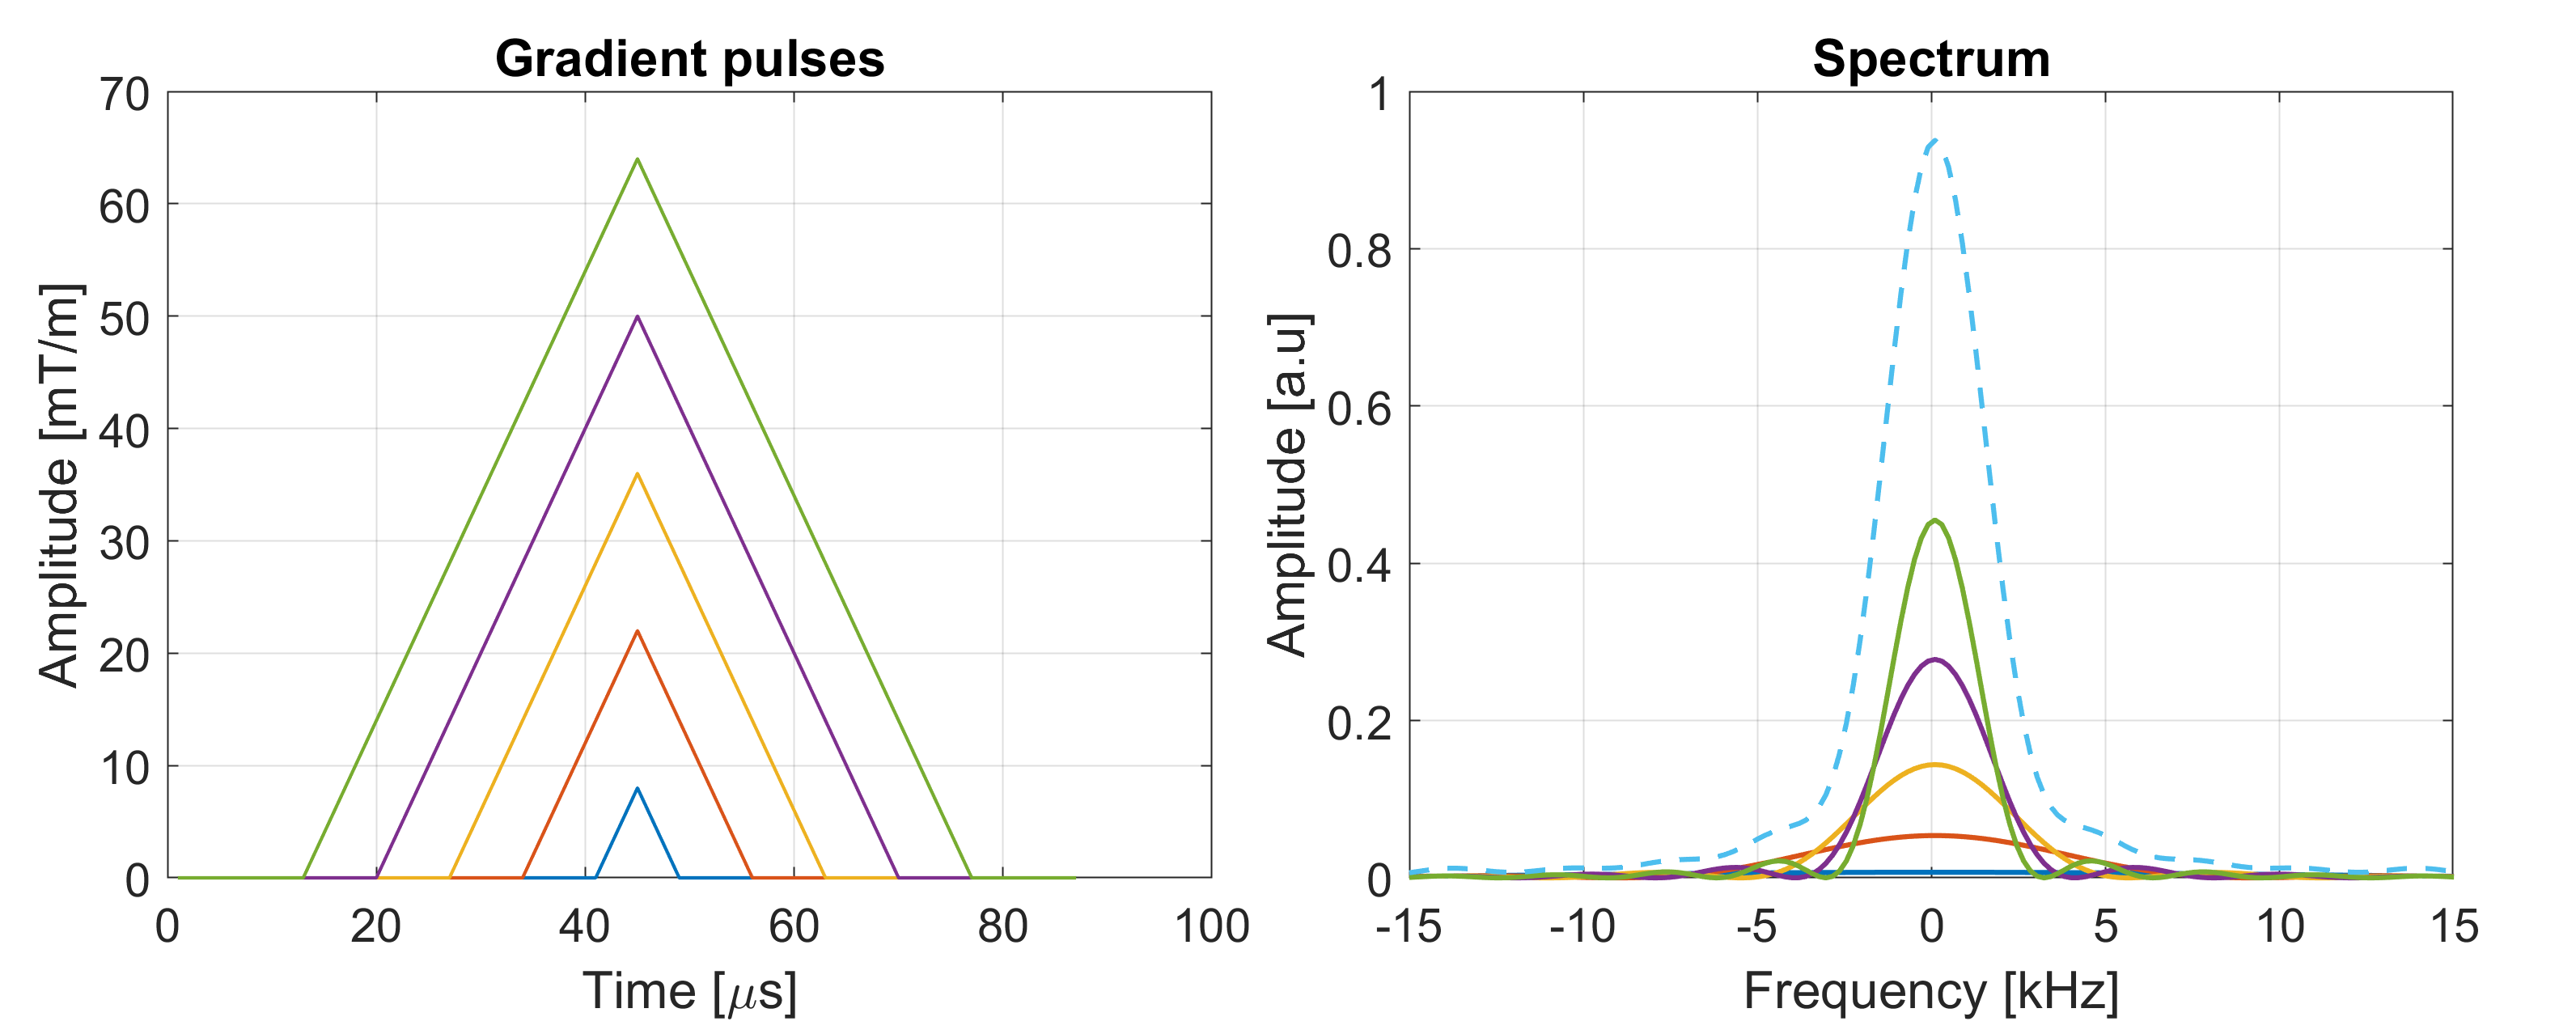
\includegraphics[width=1.0\textwidth]{graphics/GIRF.png}
	\caption{Sensitivity of gradient impulse response function (GIRF) measurement. The input triangular gradient waveform of various duration and their frequency response. }
	\label{fig:GIRF}
\end{figure}

If the input triangular pulses in Fourier domain $I_j(\omega)$ yield the system responses $\hat{O}_j(\omega)$, then the \gls{GIRF} $\hat{H}(\omega)$ can be calculated according to Vannesjo et al.\cite{vannesjoGradientSystemCharacterization2013}

\begin{equation}
	\hat{H}(\omega)=\frac{\sum_{j}I^*_j(\omega)\cdot\hat{O}_j(\omega)}{\sum_{j}|I_j(\omega)|^2}
\end{equation} 




\subsection{Spiral Deblurring}
\begin{equation}
	e^{j\Delta\omega t} \approx \sum_{i=0}^{L} c_i(\Delta\omega)e^{j\Delta\omega_it} \approx \sum_{i=0}^{L} c_i(t)e^{j\Delta\omega\tau_i}
\end{equation}

where $c_i(t)$ and $c_i(\Delta\omega)$ are the interpolation coefficients in  estimated with least-squares.

\begin{figure}[H]
	\centering
	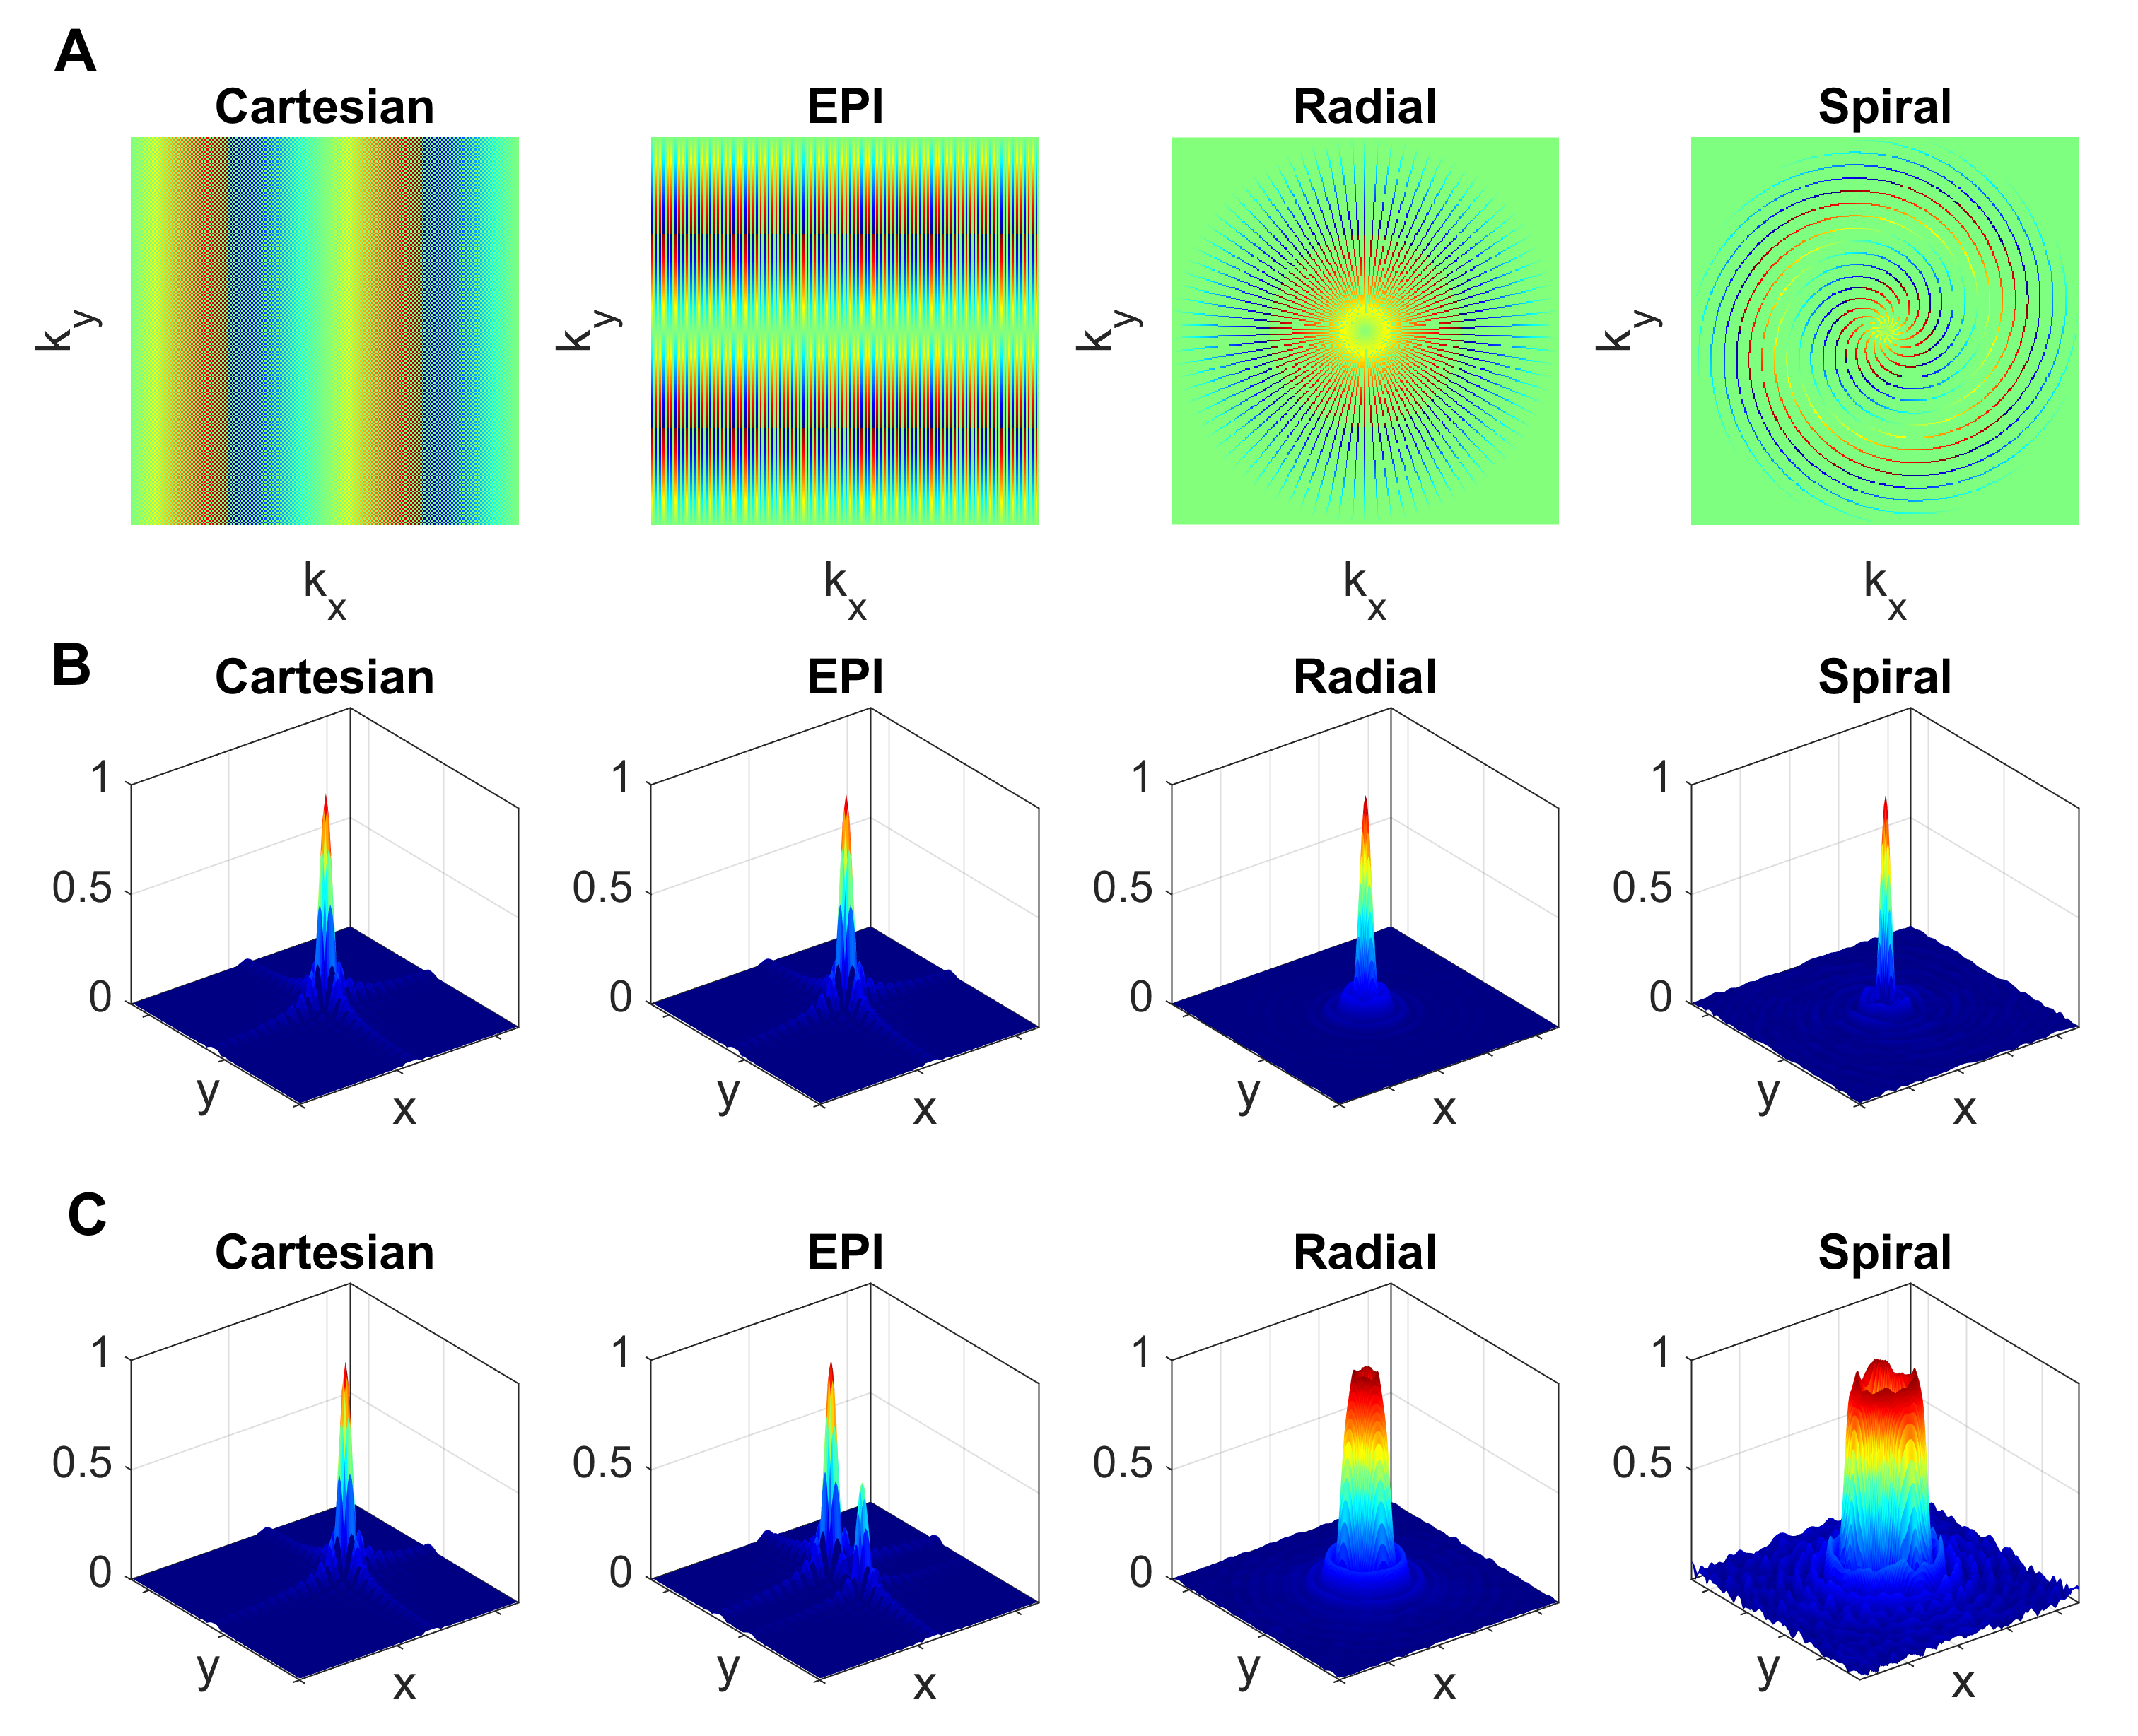
\includegraphics[width=1.0\textwidth]{graphics/spiral_psf.png}
	\caption{The influence of spatial $B_0$ off-resonance to the PSF.}
	\label{fig:spiral_psf}
\end{figure}



\subsection{Non-Cartesian Parallel imaging}

\begin{figure}[H]
	\centering
	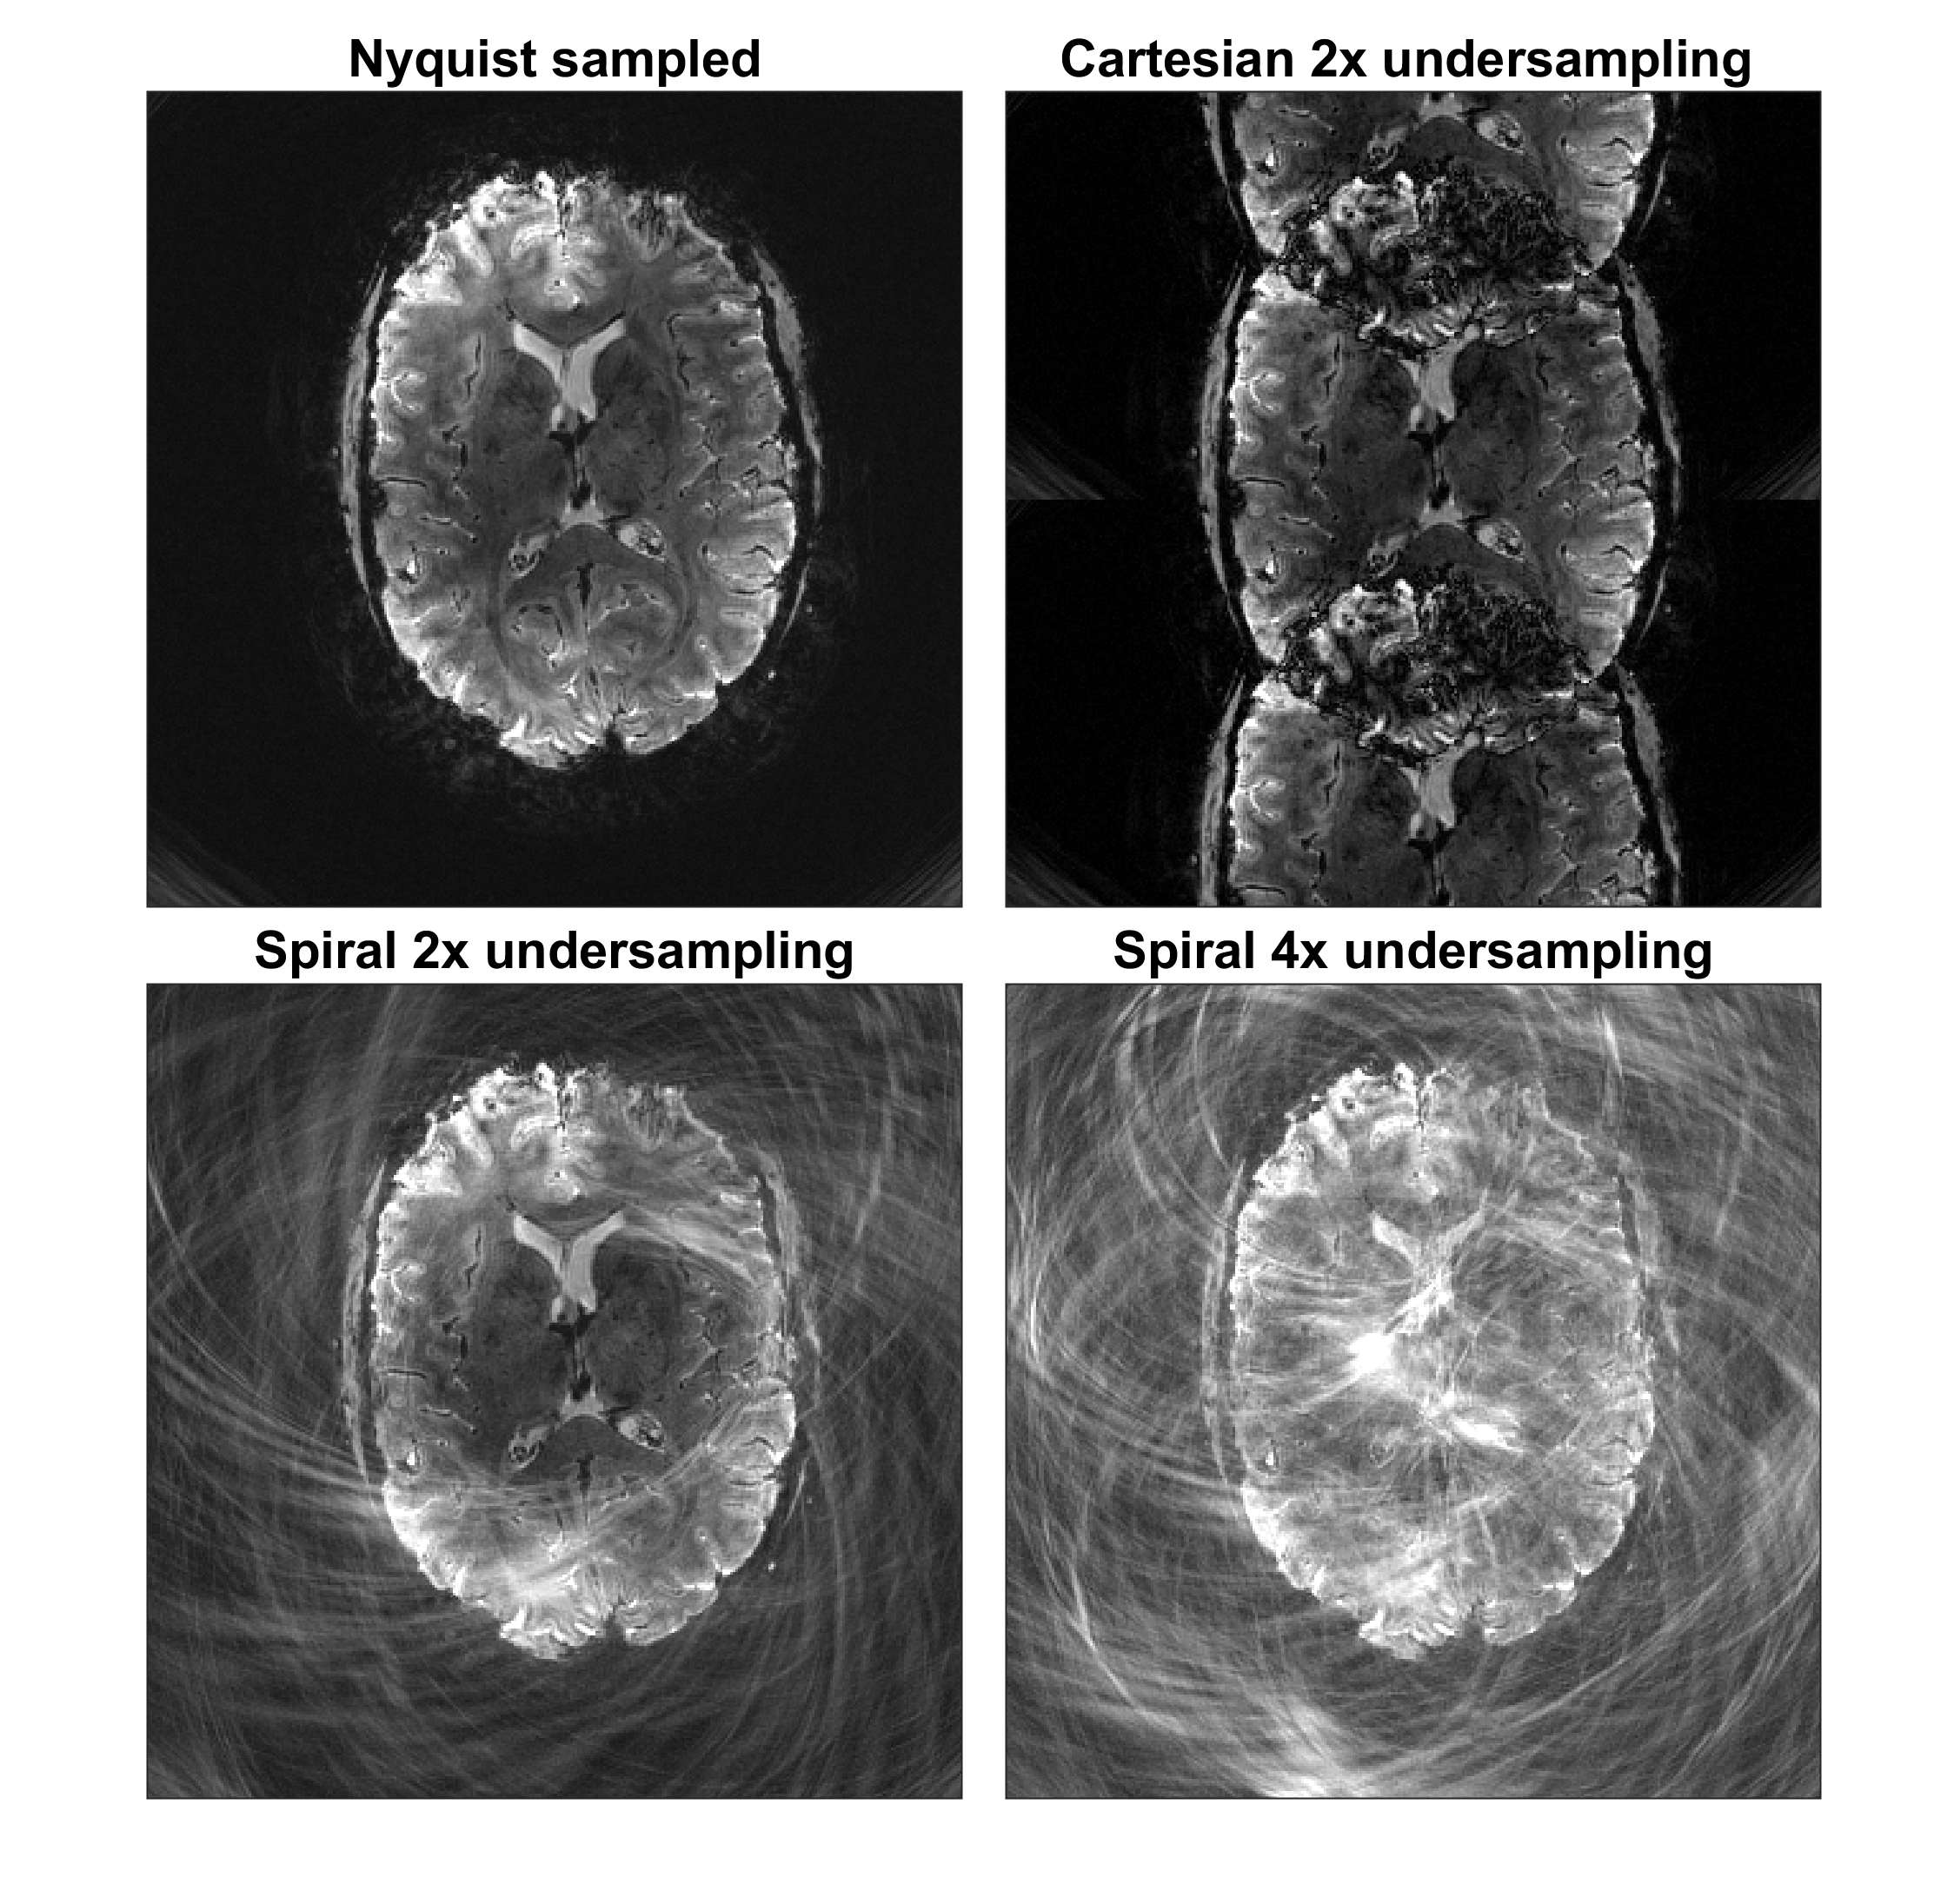
\includegraphics[width=1.0\textwidth]{graphics/Spiral_US.png}
	\caption{The undersampling artefact in Cartesian and Spiral acquisition'}
	\label{fig:ss_seq}
\end{figure}

\subsection{Iterative reconstruction}





-